% Created by tikzDevice version 0.12.6 on 2024-07-05 16:41:19
% !TEX encoding = UTF-8 Unicode
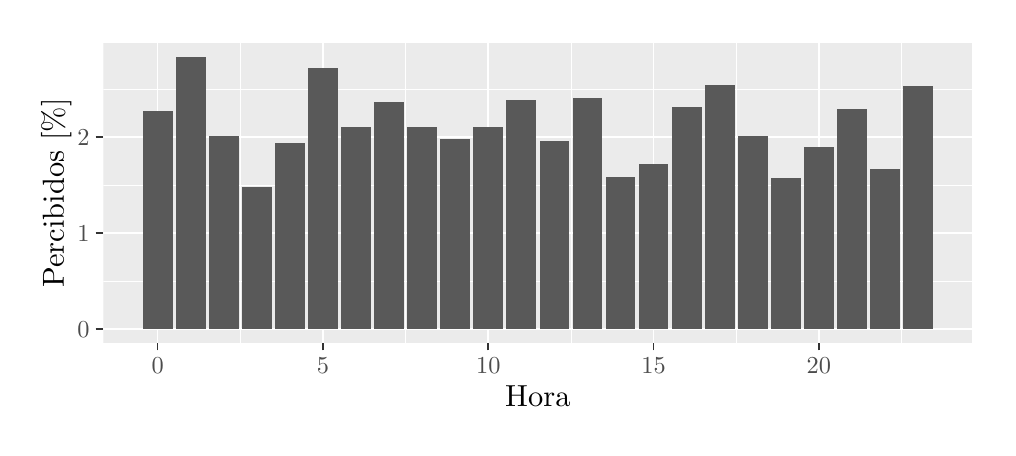
\begin{tikzpicture}[x=1pt,y=1pt]
\definecolor{fillColor}{RGB}{255,255,255}
\path[use as bounding box,fill=fillColor,fill opacity=0.00] (0,0) rectangle (346.90,144.54);
\begin{scope}
\path[clip] (  0.00,  0.00) rectangle (346.90,144.54);
\definecolor{drawColor}{RGB}{255,255,255}
\definecolor{fillColor}{RGB}{255,255,255}

\path[draw=drawColor,line width= 0.6pt,line join=round,line cap=round,fill=fillColor] (  0.00,  0.00) rectangle (346.90,144.54);
\end{scope}
\begin{scope}
\path[clip] ( 27.31, 30.69) rectangle (341.40,139.04);
\definecolor{fillColor}{gray}{0.92}

\path[fill=fillColor] ( 27.31, 30.69) rectangle (341.40,139.04);
\definecolor{drawColor}{RGB}{255,255,255}

\path[draw=drawColor,line width= 0.3pt,line join=round] ( 27.31, 52.95) --
	(341.40, 52.95);

\path[draw=drawColor,line width= 0.3pt,line join=round] ( 27.31, 87.62) --
	(341.40, 87.62);

\path[draw=drawColor,line width= 0.3pt,line join=round] ( 27.31,122.29) --
	(341.40,122.29);

\path[draw=drawColor,line width= 0.3pt,line join=round] ( 76.83, 30.69) --
	( 76.83,139.04);

\path[draw=drawColor,line width= 0.3pt,line join=round] (136.57, 30.69) --
	(136.57,139.04);

\path[draw=drawColor,line width= 0.3pt,line join=round] (196.30, 30.69) --
	(196.30,139.04);

\path[draw=drawColor,line width= 0.3pt,line join=round] (256.04, 30.69) --
	(256.04,139.04);

\path[draw=drawColor,line width= 0.3pt,line join=round] (315.77, 30.69) --
	(315.77,139.04);

\path[draw=drawColor,line width= 0.6pt,line join=round] ( 27.31, 35.61) --
	(341.40, 35.61);

\path[draw=drawColor,line width= 0.6pt,line join=round] ( 27.31, 70.28) --
	(341.40, 70.28);

\path[draw=drawColor,line width= 0.6pt,line join=round] ( 27.31,104.96) --
	(341.40,104.96);

\path[draw=drawColor,line width= 0.6pt,line join=round] ( 46.97, 30.69) --
	( 46.97,139.04);

\path[draw=drawColor,line width= 0.6pt,line join=round] (106.70, 30.69) --
	(106.70,139.04);

\path[draw=drawColor,line width= 0.6pt,line join=round] (166.43, 30.69) --
	(166.43,139.04);

\path[draw=drawColor,line width= 0.6pt,line join=round] (226.17, 30.69) --
	(226.17,139.04);

\path[draw=drawColor,line width= 0.6pt,line join=round] (285.90, 30.69) --
	(285.90,139.04);
\definecolor{fillColor}{gray}{0.35}

\path[fill=fillColor] ( 41.59, 35.61) rectangle ( 52.34,114.48);

\path[fill=fillColor] ( 53.54, 35.61) rectangle ( 64.29,134.11);

\path[fill=fillColor] ( 65.48, 35.61) rectangle ( 76.24,105.55);

\path[fill=fillColor] ( 77.43, 35.61) rectangle ( 88.18, 87.04);

\path[fill=fillColor] ( 89.38, 35.61) rectangle (100.13,102.85);

\path[fill=fillColor] (101.32, 35.61) rectangle (112.08,129.79);

\path[fill=fillColor] (113.27, 35.61) rectangle (124.02,108.55);

\path[fill=fillColor] (125.22, 35.61) rectangle (135.97,117.61);

\path[fill=fillColor] (137.16, 35.61) rectangle (147.92,108.49);

\path[fill=fillColor] (149.11, 35.61) rectangle (159.86,104.44);

\path[fill=fillColor] (161.06, 35.61) rectangle (171.81,108.48);

\path[fill=fillColor] (173.01, 35.61) rectangle (183.76,118.37);

\path[fill=fillColor] (184.95, 35.61) rectangle (195.70,103.60);

\path[fill=fillColor] (196.90, 35.61) rectangle (207.65,118.98);

\path[fill=fillColor] (208.85, 35.61) rectangle (219.60, 90.51);

\path[fill=fillColor] (220.79, 35.61) rectangle (231.54, 95.35);

\path[fill=fillColor] (232.74, 35.61) rectangle (243.49,115.94);

\path[fill=fillColor] (244.69, 35.61) rectangle (255.44,123.95);

\path[fill=fillColor] (256.63, 35.61) rectangle (267.39,105.35);

\path[fill=fillColor] (268.58, 35.61) rectangle (279.33, 90.19);

\path[fill=fillColor] (280.53, 35.61) rectangle (291.28,101.45);

\path[fill=fillColor] (292.47, 35.61) rectangle (303.23,115.02);

\path[fill=fillColor] (304.42, 35.61) rectangle (315.17, 93.40);

\path[fill=fillColor] (316.37, 35.61) rectangle (327.12,123.39);
\end{scope}
\begin{scope}
\path[clip] (  0.00,  0.00) rectangle (346.90,144.54);
\definecolor{drawColor}{gray}{0.30}

\node[text=drawColor,anchor=base east,inner sep=0pt, outer sep=0pt, scale=  0.88] at ( 22.36, 32.58) {0};

\node[text=drawColor,anchor=base east,inner sep=0pt, outer sep=0pt, scale=  0.88] at ( 22.36, 67.25) {1};

\node[text=drawColor,anchor=base east,inner sep=0pt, outer sep=0pt, scale=  0.88] at ( 22.36,101.93) {2};
\end{scope}
\begin{scope}
\path[clip] (  0.00,  0.00) rectangle (346.90,144.54);
\definecolor{drawColor}{gray}{0.20}

\path[draw=drawColor,line width= 0.6pt,line join=round] ( 24.56, 35.61) --
	( 27.31, 35.61);

\path[draw=drawColor,line width= 0.6pt,line join=round] ( 24.56, 70.28) --
	( 27.31, 70.28);

\path[draw=drawColor,line width= 0.6pt,line join=round] ( 24.56,104.96) --
	( 27.31,104.96);
\end{scope}
\begin{scope}
\path[clip] (  0.00,  0.00) rectangle (346.90,144.54);
\definecolor{drawColor}{gray}{0.20}

\path[draw=drawColor,line width= 0.6pt,line join=round] ( 46.97, 27.94) --
	( 46.97, 30.69);

\path[draw=drawColor,line width= 0.6pt,line join=round] (106.70, 27.94) --
	(106.70, 30.69);

\path[draw=drawColor,line width= 0.6pt,line join=round] (166.43, 27.94) --
	(166.43, 30.69);

\path[draw=drawColor,line width= 0.6pt,line join=round] (226.17, 27.94) --
	(226.17, 30.69);

\path[draw=drawColor,line width= 0.6pt,line join=round] (285.90, 27.94) --
	(285.90, 30.69);
\end{scope}
\begin{scope}
\path[clip] (  0.00,  0.00) rectangle (346.90,144.54);
\definecolor{drawColor}{gray}{0.30}

\node[text=drawColor,anchor=base,inner sep=0pt, outer sep=0pt, scale=  0.88] at ( 46.97, 19.68) {0};

\node[text=drawColor,anchor=base,inner sep=0pt, outer sep=0pt, scale=  0.88] at (106.70, 19.68) {5};

\node[text=drawColor,anchor=base,inner sep=0pt, outer sep=0pt, scale=  0.88] at (166.43, 19.68) {10};

\node[text=drawColor,anchor=base,inner sep=0pt, outer sep=0pt, scale=  0.88] at (226.17, 19.68) {15};

\node[text=drawColor,anchor=base,inner sep=0pt, outer sep=0pt, scale=  0.88] at (285.90, 19.68) {20};
\end{scope}
\begin{scope}
\path[clip] (  0.00,  0.00) rectangle (346.90,144.54);
\definecolor{drawColor}{RGB}{0,0,0}

\node[text=drawColor,anchor=base,inner sep=0pt, outer sep=0pt, scale=  1.10] at (184.35,  7.64) {Hora};
\end{scope}
\begin{scope}
\path[clip] (  0.00,  0.00) rectangle (346.90,144.54);
\definecolor{drawColor}{RGB}{0,0,0}

\node[text=drawColor,rotate= 90.00,anchor=base,inner sep=0pt, outer sep=0pt, scale=  1.10] at ( 13.08, 84.86) {Percibidos [\%]};
\end{scope}
\end{tikzpicture}
